% Please make sure you insert your
% data according to the instructions in PoSauthmanual.pdf
\documentclass[a4paper,11pt]{article}
\usepackage{pos}
\usepackage{xspace}
\usepackage{subcaption}

\title{\euclid's Sensitivity to Neutrino Parameters}
%% \ShortTitle{Short Title for header}

\newcommand{\euclid}{\textit{Euclid}\xspace}
\newcommand{\planck}{\textit{Planck}\xspace}

\newcommand{\dneff}{\Delta N_\mathrm{eff}}
\newcommand{\summnu}{\sum m_\nu}

\newcommand{\threetimestwo}{3$\times$2\,pt}

\newcommand{\camb}{\texttt{CAMB}\xspace}
\newcommand{\class}{\texttt{CLASS}\xspace}
\newcommand{\montepython}{\texttt{MontePython}\xspace}
\newcommand{\cosmicfish}{\texttt{CosmicFish}\xspace}

\newcommand*\aap{A\&A}
\let\astap=\aap
\newcommand*\aapr{A\&A~Rev.}
\newcommand*\aaps{A\&AS}
\newcommand*\actaa{Acta Astron.}
\newcommand*\aj{AJ}
\newcommand*\ao{Appl.~Opt.}
\let\applopt\ao
\newcommand*\apj{ApJ}
\newcommand*\apjl{ApJ}
\let\apjlett\apjl
\newcommand*\apjs{ApJS}
\let\apjsupp\apjs
\newcommand*\aplett{Astrophys.~Lett.}
\newcommand*\apspr{Astrophys.~Space~Phys.~Res.}
\newcommand*\apss{Ap\&SS}
\newcommand*\araa{ARA\&A}
\newcommand*\azh{AZh}
\newcommand*\baas{BAAS}
\newcommand*\bac{Bull. astr. Inst. Czechosl.}
\newcommand*\bain{Bull.~Astron.~Inst.~Netherlands}
\newcommand*\caa{Chinese Astron. Astrophys.}
\newcommand*\cjaa{Chinese J. Astron. Astrophys.}
\newcommand*\fcp{Fund.~Cosmic~Phys.}
\newcommand*\gca{Geochim.~Cosmochim.~Acta}
\newcommand*\grl{Geophys.~Res.~Lett.}
\newcommand*\iaucirc{IAU~Circ.}
\newcommand*\icarus{Icarus}
\newcommand*\jcap{J. Cosmology Astropart. Phys.}
\newcommand*\jcp{J.~Chem.~Phys.}
\newcommand*\jgr{J.~Geophys.~Res.}
\newcommand*\jqsrt{J.~Quant.~Spectr.~Rad.~Transf.}
\newcommand*\jrasc{JRASC}
\newcommand*\memras{MmRAS}
\newcommand*\memsai{Mem.~Soc.~Astron.~Italiana}
\newcommand*\mnras{MNRAS}
\newcommand*\na{New A}
\newcommand*\nar{New A Rev.}
\newcommand*\nat{Nature}
\newcommand*\nphysa{Nucl.~Phys.~A}
\newcommand*\pasa{PASA}
\newcommand*\pasj{PASJ}
\newcommand*\pasp{PASP}
\newcommand*\physrep{Phys.~Rep.}
\newcommand*\physscr{Phys.~Scr}
\newcommand*\planss{Planet.~Space~Sci.}
\newcommand*\pra{Phys.~Rev.~A}
\newcommand*\prb{Phys.~Rev.~B}
\newcommand*\prc{Phys.~Rev.~C}
\newcommand*\prd{Phys.~Rev.~D}
\newcommand*\pre{Phys.~Rev.~E}
\newcommand*\prl{Phys.~Rev.~Lett.}
\newcommand*\procspie{Proc.~SPIE}
\newcommand*\qjras{QJRAS}
\newcommand*\rmxaa{Rev. Mexicana Astron. Astrofis.}
\newcommand*\skytel{S\&T}
\newcommand*\solphys{Sol.~Phys.}
\newcommand*\sovast{Soviet~Ast.}
\newcommand*\ssr{Space~Sci.~Rev.}
\newcommand*\zap{ZAp}

\author[1,2]{ M.~Archidiacono}
\author[3]{ J.~Lesgourgues}
\author[3]{ S.~Casas}
\author*[4]{ S.~Pamuk}
\author[5]{ N.~Sch\"oneberg}
\author[6,7,8]{ Z.~Sakr}
\author[9,10,11]{ G.~Parimbelli}
\author[12]{ A.~Schneider}
\author[13,12]{ F.~Hervas~Peters}
\author[14,15,16]{ F.~Pace}
\author[3,17]{ V.~M.~Sabarish}
\author[18,19,20]{ M.~Costanzi}
\author[14,15,16]{ S.~Camera}
\author[21]{ C.~Carbone}
\author[22]{ S.~Clesse}
\author[23]{ N.~Frusciante}
\author[24,20]{ A.~Fumagalli}
\author[18,19,25,20]{ P.~Monaco}
\author[26]{ D.~Scott}
\author[19,18,10,24,27]{ M.~Viel}

\affiliation[1]{Dipartimento di Fisica "Aldo Pontremoli", Universit\`a degli Studi di Milano, Via Celoria 16, 20133 Milano, Italy}
\affiliation[2]{INFN-Sezione di Milano, Via Celoria 16, 20133 Milano, Italy}
\affiliation[3]{Institute for Theoretical Particle Physics and Cosmology (TTK), RWTH Aachen University, 52056 Aachen, Germany}
\affiliation[4]{Instituto de F\'{\i}sica de Cantabria (IFCA), CSIC-Univ. de Cantabria, Avda. de los Castros s/n, E-39005 Santander, Spain}
\affiliation[5]{Institut de Ci\`{e}ncies del Cosmos (ICCUB), Universitat de Barcelona (IEEC-UB), Mart\'{i} i Franqu\`{e}s 1, 08028 Barcelona, Spain}
\affiliation[6]{Institut f\"ur Theoretische Physik, University of Heidelberg, Philosophenweg 16, 69120 Heidelberg, Germany}
\affiliation[7]{Institut de Recherche en Astrophysique et Plan\'etologie (IRAP), Universit\'e de Toulouse, CNRS, UPS, CNES, 14 Av. Edouard Belin, 31400 Toulouse, France}
\affiliation[8]{Universit\'e St Joseph; Faculty of Sciences, Beirut, Lebanon}
\affiliation[9]{Institute of Space Sciences (ICE, CSIC), Campus UAB, Carrer de Can Magrans, s/n, 08193 Barcelona, Spain}
\affiliation[10]{Dipartimento di Fisica, Universit\`a degli studi di Genova, and INFN-Sezione di Genova, via Dodecaneso 33, 16146, Genova, Italy}
\affiliation[11]{SISSA, International School for Advanced Studies, Via Bonomea 265, 34136 Trieste TS, Italy}
\affiliation[12]{Department of Astrophysics, University of Zurich, Winterthurerstrasse 190, 8057 Zurich, Switzerland}
\affiliation[13]{Université Paris-Saclay, Université Paris Cité, CEA, CNRS, AIM, 91191, Gif-sur-Yvette, France}
\affiliation[14]{Dipartimento di Fisica, Universit\`a degli Studi di Torino, Via P. Giuria 1, 10125 Torino, Italy}
\affiliation[15]{INFN-Sezione di Torino, Via P. Giuria 1, 10125 Torino, Italy}
\affiliation[16]{INAF-Osservatorio Astrofisico di Torino, Via Osservatorio 20, 10025 Pino Torinese (TO), Italy}
\affiliation[17]{Hamburger Sternwarte, University of Hamburg, Gojenbergsweg 112, 21029 Hamburg, Germany}
\affiliation[18]{Dipartimento di Fisica - Sezione di Astronomia, Universit\`a di Trieste, Via Tiepolo 11, 34131 Trieste, Italy}
\affiliation[19]{INAF-Osservatorio Astronomico di Trieste, Via G. B. Tiepolo 11, 34143 Trieste, Italy}
\affiliation[20]{IFPU, Institute for Fundamental Physics of the Universe, via Beirut 2, 34151 Trieste, Italy}
\affiliation[21]{INAF-IASF Milano, Via Alfonso Corti 12, 20133 Milano, Italy}
\affiliation[22]{Universit\'e Libre de Bruxelles (ULB), Service de Physique Th\'eorique CP225, Boulevard du Triophe, 1050 Bruxelles, Belgium}
\affiliation[23]{Department of Physics "E. Pancini", University Federico II, Via Cinthia 6, 80126, Napoli, Italy}
\affiliation[24]{Ludwig-Maximilians-University, Schellingstrasse 4, 80799 Munich, Germany}
\affiliation[25]{INFN, Sezione di Trieste, Via Valerio 2, 34127 Trieste TS, Italy}
\affiliation[26]{Department of Physics and Astronomy, University of British Columbia, Vancouver, BC V6T 1Z1, Canada}
\affiliation[27]{ICSC - Centro Nazionale di Ricerca in High Performance Computing, Big Data e Quantum Computing, Via Magnanelli 2, Bologna, Italy}

\emailAdd{pamuk@ifca.unican.es}

\abstract{The European Space Agency launched its newest mission in July 2023: \euclid, which is designed to create the largest galaxy clustering and weak gravitational lensing survey to date. The complementarity of wide imaging and spectroscopy will provide excellent sensitivity to the history of structure formation, and hence to physics that affects that history.
Here we present the latest forecasts of how \euclid's main cosmological probes will be able to constrain parameters from neutrino physics. Specifically we focus on the summed mass of neutrino species $\summnu$, as well as the effective number of additional relativistic species $\dneff$.
We show how the forthcoming \euclid data should lead to unprecedented sensitivity for these parameters, and together with data from future cosmic microwave background experiments, could enable a detection of the neutrino mass scale.
%The work presented here is based on Archidiacono et al.~\cite{EP-Archidiacono}.
}

\FullConference{12th Neutrino Oscillation Workshop (NOW2024)\\
 2-8, September 2024\\
Otranto, Lecce, Italy\\}

\newcommand*{\AckInstitutions}{a number of agencies and
  institutes that have supported the development of \euclid, in
  particular
  the Agenzia Spaziale Italiana,
  the Austrian Forschungsf\"orderungsgesellschaft funded through BMK,
  the Belgian Science Policy,
  the Canadian Euclid Consortium,
  the Deutsches Zentrum f\"ur Luft- und Raumfahrt,
  the DTU Space and the Niels Bohr Institute in Denmark,
  the French Centre National d'Etudes Spatiales,
  the Funda\c{c}\~{a}o para a Ci\^{e}ncia e a Tecnologia,
  the Hungarian Academy of Sciences,
  the Ministerio de Ciencia, Innovaci\'{o}n y Universidades,
  the National Aeronautics and Space Administration,
  the National Astronomical Observatory of Japan,
  the Netherlandse Onderzoekschool Voor Astronomie,
  the Norwegian Space Agency,
  the Research Council of Finland,
  the Romanian Space Agency,
  the State Secretariat for Education, Research, and Innovation (SERI) at the Swiss
  Space Office (SSO),
  and the United Kingdom Space Agency.
  A complete and detailed list is available on the \euclid\ web site
  (\url{www.euclid-ec.org}).\xspace}
\newcommand{\AckEC}{The Euclid Consortium acknowledges the European
  Space Agency and \AckInstitutions}

%% \tableofcontents

\begin{document}
\maketitle


\section{Background}
The \euclid mission\cite{EuclidSkyOverview} will measure the locations and shapes of more than a billion galaxies over approximately one third of the sky. \euclid will produce the largest galaxy catalogue to date,
covering lookback times of roughly ten billion years. The cosmological information that can be obtained from this data set will be used to probe the dark components of the Universe.  In terms of cosmological neutrinos, \euclid will constrain the sum of the masses, $\sum m_\nu$, as well as the effective number of extra relativistic relics, $\Delta N_\mathrm{eff}$. The effect of these quantities on cosmological observables is described in Refs.~\cite{ParticleDataGroup:2024cfk, Vagnozzi_2018, Blanchard-EP7}.

The \euclid probe that most strongly constrains $\sum m_\nu$ is the weak lensing (WL) of galaxies.
The shapes of background (source) galaxies correlate with each other because they are lensed by the same foreground (lens) halos. This shape correlation can be directly related to the underlying matter field. Adding massive neutrinos suppresses this correlation in a scale-dependent way, since it slows down the formation of structure for scales that enter the Hubble horizon while neutrinos are still too hot to cluster inside gravitational wells. Measuring the WL signal gives a unique method to directly determine the overall amplitude of the matter perturbations.

The \euclid probe that most strongly constrains $\dneff$ is galaxy clustering (GC), where the spatial correlation of galaxies is measured. The 2-point correlation function shows an excess at a particular scale, originating from expanding acoustic waves in the primordial plasma. The angular size of these baryonic acoustic oscillations (BAOs) is determined by the Universe's expansion history. This is why adding additional massless relics through $\dneff$ creates a measurable change in the BAO scale.

In addition to the BAO feature, the amplitude of the GC signal is also given by the underlying matter distribution. Since galaxies form in overdense regions, an enhancement in the density of galaxies is related to an enhancement in the total matter density. However, unlike the WL signal, this relation is not a direct correspondence, rather the galaxy field is a biased tracer of the matter field. On its own, the GC probe will only be able to measure the amplitude of matter perturbations in combination with parameters describing this bias.  \euclid will be able to construct the GC power spectrum using photometric redshifts, as well as using spectroscopic ones; we denote these photometric and spectroscopic clustering probes as GCph and GCsp, respectively. While the galaxies for which we have measured photometric redshifts will mainly be used by binning them into 2-dimensional slices in redshift, the spectroscopic redshift measurements will allow for the computation of the 3-dimensional redshift-space power spectrum. GCsp also contains redshift-space distortions(RSDs), which have an additional cosmology dependence. 

The combination of the WL and GC probes can be used to break parameter degeneracies, since they measure different tracers (the gravitational potential and the clustered matter, respectively), which are affected in a different way by $\dneff$ and $\summnu$. From all of these probes, we construct 2-point statistics. Given that the intervening lenses for WL are associated with clustered galaxies, it is natural to expect a cross-correlation (XC) between the WL and GCph probes, i.e., an additional 2-point statistic.  In addition to \euclid's probes
we can add information from the cosmic microwave background (CMB) to further constrain neutrino parameters.

\section{Methodology}

The forecasts were performed using Markov chain Monte Carlo (MCMC) methods to go beyond the standard Fisher information (FI) formalism. This is because we expect deviations from Gaussian posteriors for the neutrino parameters, as well as applying the additional physical constraint of a positive neutrino mass.

Our forecast validation was carried out in three distinct steps. In the first step, we validated our Einstein--Boltzmann solver (EBS) by performing multiple FI forecasts, where we have compared different solvers. For this purpose, we used the \cosmicfish code that was validated before within the efforts of the Euclid Consortium \cite{Blanchard-EP7}. The two most common EBSs are \camb \cite{2011ascl.soft02026L} and \class \cite{Diego_Blas_2011}. While their agreement has been established for past CMB and LSS experiments, the new frontier of precision unlocked by \euclid needed a new validation at higher precision. Furthermore, the \euclid observables will require us to have good control of the nonlinear corrections to the power spectrum. We performed a thorough analysis of multiple recipes for these nonlinear corrections and compared them to $N$-body simulations. In the presence of massive neutrinos, the best comparison was achieved with the \texttt{HMCode2020} recipe \cite{Mead_2021}. In this way, the \texttt{HMCode2020} recipes within \class and \camb were validated for the first time.

We then constructed a likelihood for \montepython \cite{Audren:2012wb} as an extension of the existing likelihood formulated in Ref.~\cite{Casas23}. The modelling of the galaxy bias needs particular care in the presence of massive neutrinos, otherwise this can bias the measured value and sensitivity for $\summnu$ \cite{Vagnozzi_2018}. Since neutrinos do not cluster inside halos, the RSDs are driven by cold dark matter and baryonic matter only \cite{Villaescusa_Navarro_2018}. For this reason, the measured signal has to be additionally modified to describe this effect. In the second step, we validated our likelihood by performing an FI forecast with it and compared the results to those from the first step.

Finally, we ran an MCMC simulation using our \montepython likelihood to check for the validity of our FI forecast. We observed deviations between MCMC and FI that could be explained by non-Gaussianities of the posterior, as well as from prior effects. This confirms the necessity of using MCMC methods. 

\section{Results}

The final forecast was performed using \montepython. We varied different sets of cosmological parameters for the analysis to study how much the constraints degrade by opening up the parameter space. The baseline model consists of five $\varLambda$CDM parameters, as well as $\summnu$, i.e., \{$h$, $\Omega_\mathrm{m}$, $\Omega_\mathrm{b}$, $\sigma_8$, $n_\mathrm{s}$, $\summnu$\}. We also studied what happens when opening up the number of additional massless relics \{$\dneff$\}, and/or the Chevallier--Polarski--Linder parameters for the equation of state of dark energy \{$w_0,w_a$\}. Additionally, when adding information from CMB experiments we varied the optical depth of reionisation \{$\tau$\}. We assumed a spatially flat cosmology and three massive neutrinos with degenerate masses. It was shown that the latter choice is appropriate because individual mass splittings are not resolvable with cosmological data \cite{Lesgourgues:2013sjj}.

We performed these forecasts for different combinations of the \euclid cosmology probes, as well as adding additional constraints from CMB experiments. For the survey specifications of \euclid we used the `pessimistic' settings outlined in Ref.~\cite{Blanchard-EP7}. We consider two cases for the CMB experiments: a mock likelihood for \planck \cite{Planck:2018vyg}; and a future setup of CMB-S4 \cite{CMBS4} + LiteBird \cite{LiteBIRD}.

For the combination of the main \euclid probes we find in the baseline model a sensitivity to the cosmological neutrino mass of $\sigma\left(\summnu\right)=56\,\mathrm{meV}$. This degrades to a 95\% confidence level (CL) of $\summnu<220\,\mathrm{meV}$ when opening up $\dneff$. The distribution is non-Gaussian due to the prior edge, and therefore we report the upper bound. For $\dneff$ we find $\dneff<0.746$ (95\% CL). Opening up the dark energy equation of state does not measurably degrade the sensitivity to $\summnu$, while the limit on $\dneff$ degrades to $<0.935$ (95\% CL).  

Adding CMB data tightens the constraints in the full 10-parameter model to \mbox{$\sigma\left(\summnu\right)=40\,\mathrm{meV}$} or $\sigma\left(\summnu\right)=31\,\mathrm{meV}$ for \planck or CMB-S4+LiteBird, respectively. The constraints on $\dneff$ are dominated by CMB probes, but the main degeneracy of $\dneff$ with the Hubble constant is broken using the \euclid data. The combination of \euclid and CMB data could provide unprecedented sensitivity to $\dneff$, with a forecast sensitivity of $\dneff<0.149$ or $\dneff<0.069$ for \euclid + \planck or \euclid + CMB-S4 + LiteBird, respectively. 

These forecast sensitivities are placed into  context in Fig.~\ref{fig:results}, taken from Archidiacono et al.~\cite{EP-Archidiacono}. We show how for the minimal mass scenario \euclid + CMB should be able to significantly stress the inverted hierarchy model. Additionally, this combination will be able to exclude the most common types of dark relics with early (pre-QCD phase transition) injection.   

\begin{figure}[!htbp]
    \centering
    \begin{subfigure}{0.49\textwidth}
        \centering
        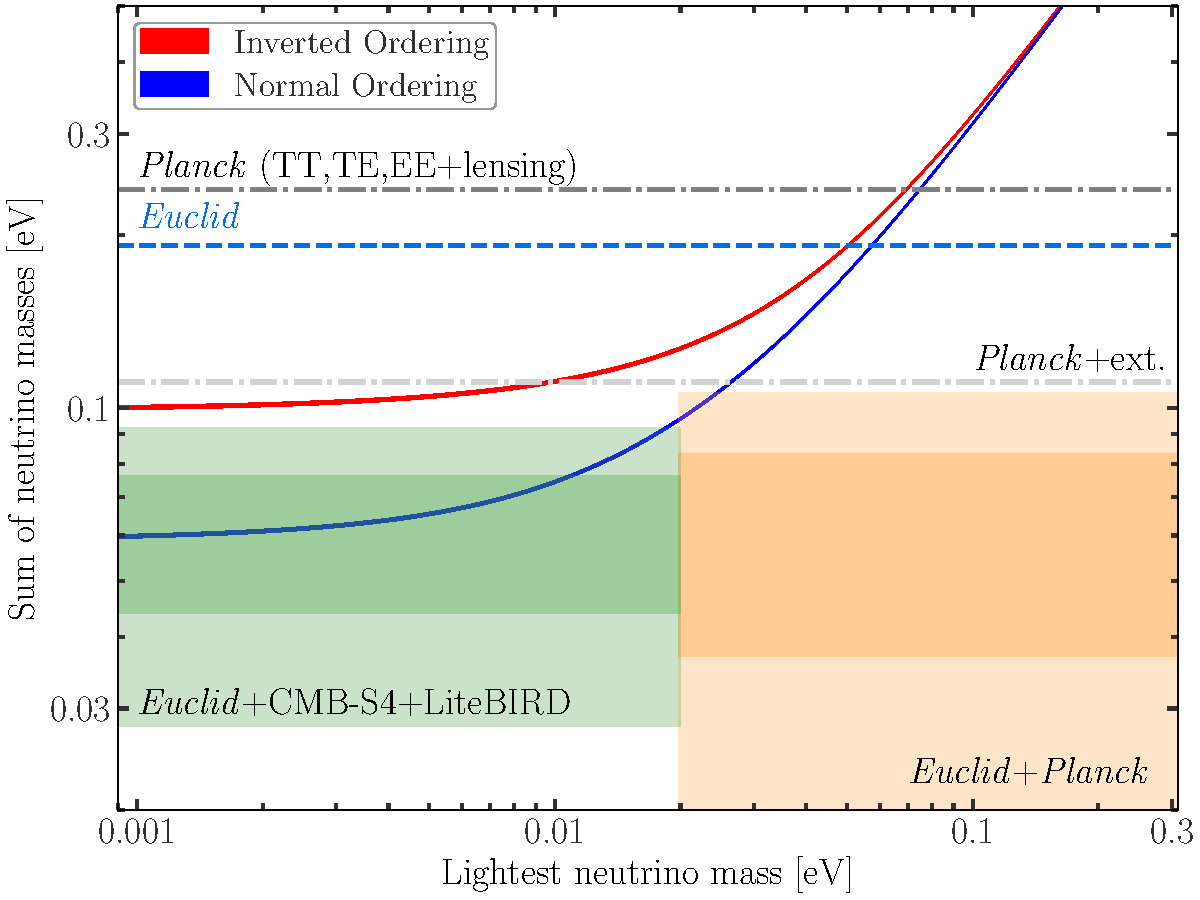
\includegraphics[width=\linewidth]{figure_hierarchy-1.pdf}
    \end{subfigure}
    \hfill
    \begin{subfigure}{0.49\textwidth}
        \centering
        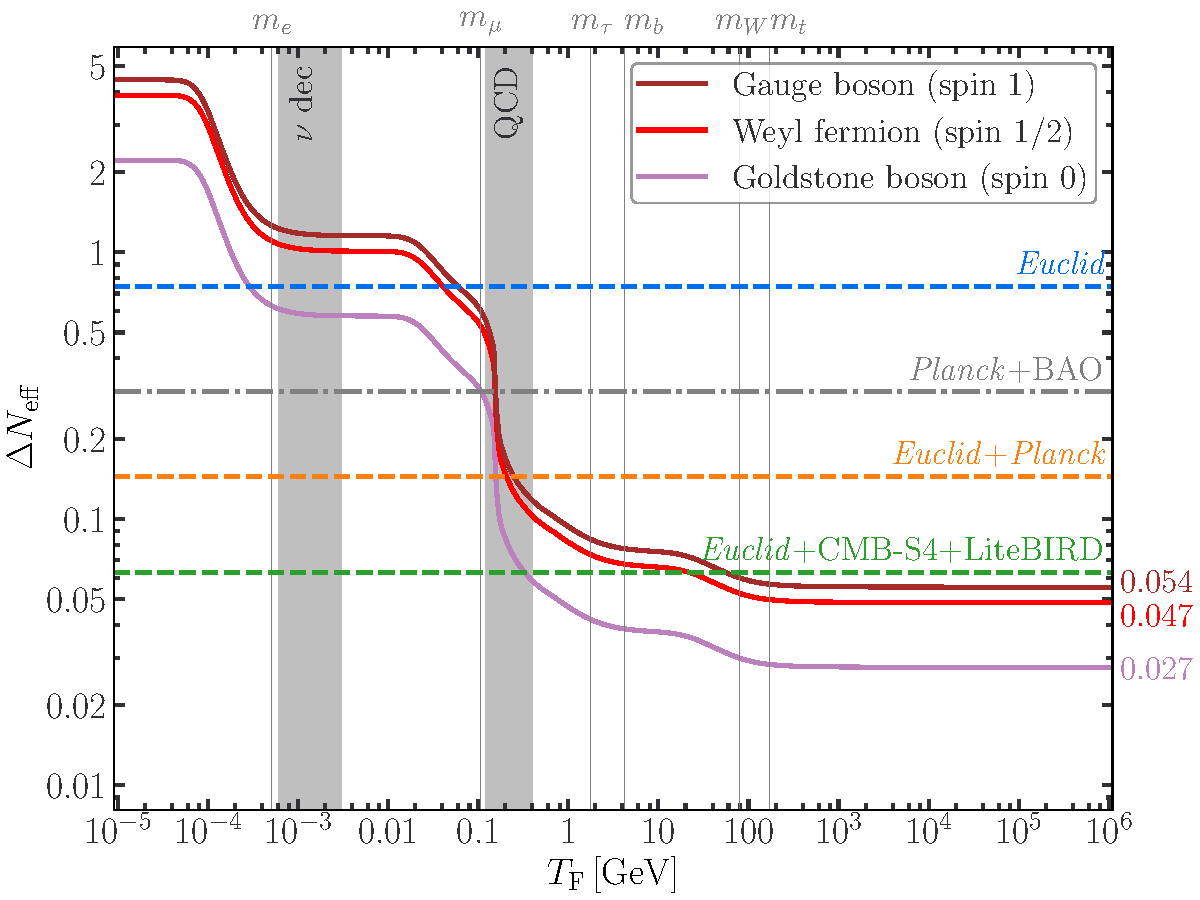
\includegraphics[width=\linewidth]{figure_Neff-1.pdf}
    \end{subfigure}
    \caption{\emph{Left}: forecast sensitivity on $\summnu$ for different combinations of \euclid, with or without CMB data. We compare the sensitivities to current measurements of \planck or \planck + additional data from supernovae, BAO measurements, and current large-scale structure measurements. The dashed lines represent the 95\% CL. The strike-through lines represent the sum of the neutrino masses from oscillation experiments, depending on the ordering and the lowest neutrino mass.
    \emph{Right}: similar to the left plot, but for the sensitivity for $\dneff$. The strike-through lines represent contributions to $\dneff$ from different types of particle and different decoupling temperatures.
    Both figures are taken from Ref.~\cite{EP-Archidiacono}.
    }
    \label{fig:results}
\end{figure}
\clearpage
\textit{Acknowledgements}: \AckEC

\bibliographystyle{JHEP}
\bibliography{my-bib-database}

\end{document}
